\documentclass[]{book}
\usepackage{lmodern}
\usepackage{amssymb,amsmath}
\usepackage{ifxetex,ifluatex}
\usepackage{fixltx2e} % provides \textsubscript
\ifnum 0\ifxetex 1\fi\ifluatex 1\fi=0 % if pdftex
  \usepackage[T1]{fontenc}
  \usepackage[utf8]{inputenc}
\else % if luatex or xelatex
  \ifxetex
    \usepackage{mathspec}
  \else
    \usepackage{fontspec}
  \fi
  \defaultfontfeatures{Ligatures=TeX,Scale=MatchLowercase}
\fi
% use upquote if available, for straight quotes in verbatim environments
\IfFileExists{upquote.sty}{\usepackage{upquote}}{}
% use microtype if available
\IfFileExists{microtype.sty}{%
\usepackage{microtype}
\UseMicrotypeSet[protrusion]{basicmath} % disable protrusion for tt fonts
}{}
\usepackage[margin=1in]{geometry}
\usepackage{hyperref}
\hypersetup{unicode=true,
            pdftitle={A Reproducible Research Compendium},
            pdfauthor={cf.~list of contributors at https://github.com/rr-mrc-bsu/reproducible-research/graphs/contributors},
            pdfborder={0 0 0},
            breaklinks=true}
\urlstyle{same}  % don't use monospace font for urls
\usepackage{natbib}
\bibliographystyle{apalike}
\usepackage{color}
\usepackage{fancyvrb}
\newcommand{\VerbBar}{|}
\newcommand{\VERB}{\Verb[commandchars=\\\{\}]}
\DefineVerbatimEnvironment{Highlighting}{Verbatim}{commandchars=\\\{\}}
% Add ',fontsize=\small' for more characters per line
\usepackage{framed}
\definecolor{shadecolor}{RGB}{248,248,248}
\newenvironment{Shaded}{\begin{snugshade}}{\end{snugshade}}
\newcommand{\KeywordTok}[1]{\textcolor[rgb]{0.13,0.29,0.53}{\textbf{#1}}}
\newcommand{\DataTypeTok}[1]{\textcolor[rgb]{0.13,0.29,0.53}{#1}}
\newcommand{\DecValTok}[1]{\textcolor[rgb]{0.00,0.00,0.81}{#1}}
\newcommand{\BaseNTok}[1]{\textcolor[rgb]{0.00,0.00,0.81}{#1}}
\newcommand{\FloatTok}[1]{\textcolor[rgb]{0.00,0.00,0.81}{#1}}
\newcommand{\ConstantTok}[1]{\textcolor[rgb]{0.00,0.00,0.00}{#1}}
\newcommand{\CharTok}[1]{\textcolor[rgb]{0.31,0.60,0.02}{#1}}
\newcommand{\SpecialCharTok}[1]{\textcolor[rgb]{0.00,0.00,0.00}{#1}}
\newcommand{\StringTok}[1]{\textcolor[rgb]{0.31,0.60,0.02}{#1}}
\newcommand{\VerbatimStringTok}[1]{\textcolor[rgb]{0.31,0.60,0.02}{#1}}
\newcommand{\SpecialStringTok}[1]{\textcolor[rgb]{0.31,0.60,0.02}{#1}}
\newcommand{\ImportTok}[1]{#1}
\newcommand{\CommentTok}[1]{\textcolor[rgb]{0.56,0.35,0.01}{\textit{#1}}}
\newcommand{\DocumentationTok}[1]{\textcolor[rgb]{0.56,0.35,0.01}{\textbf{\textit{#1}}}}
\newcommand{\AnnotationTok}[1]{\textcolor[rgb]{0.56,0.35,0.01}{\textbf{\textit{#1}}}}
\newcommand{\CommentVarTok}[1]{\textcolor[rgb]{0.56,0.35,0.01}{\textbf{\textit{#1}}}}
\newcommand{\OtherTok}[1]{\textcolor[rgb]{0.56,0.35,0.01}{#1}}
\newcommand{\FunctionTok}[1]{\textcolor[rgb]{0.00,0.00,0.00}{#1}}
\newcommand{\VariableTok}[1]{\textcolor[rgb]{0.00,0.00,0.00}{#1}}
\newcommand{\ControlFlowTok}[1]{\textcolor[rgb]{0.13,0.29,0.53}{\textbf{#1}}}
\newcommand{\OperatorTok}[1]{\textcolor[rgb]{0.81,0.36,0.00}{\textbf{#1}}}
\newcommand{\BuiltInTok}[1]{#1}
\newcommand{\ExtensionTok}[1]{#1}
\newcommand{\PreprocessorTok}[1]{\textcolor[rgb]{0.56,0.35,0.01}{\textit{#1}}}
\newcommand{\AttributeTok}[1]{\textcolor[rgb]{0.77,0.63,0.00}{#1}}
\newcommand{\RegionMarkerTok}[1]{#1}
\newcommand{\InformationTok}[1]{\textcolor[rgb]{0.56,0.35,0.01}{\textbf{\textit{#1}}}}
\newcommand{\WarningTok}[1]{\textcolor[rgb]{0.56,0.35,0.01}{\textbf{\textit{#1}}}}
\newcommand{\AlertTok}[1]{\textcolor[rgb]{0.94,0.16,0.16}{#1}}
\newcommand{\ErrorTok}[1]{\textcolor[rgb]{0.64,0.00,0.00}{\textbf{#1}}}
\newcommand{\NormalTok}[1]{#1}
\usepackage{longtable,booktabs}
\usepackage{graphicx,grffile}
\makeatletter
\def\maxwidth{\ifdim\Gin@nat@width>\linewidth\linewidth\else\Gin@nat@width\fi}
\def\maxheight{\ifdim\Gin@nat@height>\textheight\textheight\else\Gin@nat@height\fi}
\makeatother
% Scale images if necessary, so that they will not overflow the page
% margins by default, and it is still possible to overwrite the defaults
% using explicit options in \includegraphics[width, height, ...]{}
\setkeys{Gin}{width=\maxwidth,height=\maxheight,keepaspectratio}
\IfFileExists{parskip.sty}{%
\usepackage{parskip}
}{% else
\setlength{\parindent}{0pt}
\setlength{\parskip}{6pt plus 2pt minus 1pt}
}
\setlength{\emergencystretch}{3em}  % prevent overfull lines
\providecommand{\tightlist}{%
  \setlength{\itemsep}{0pt}\setlength{\parskip}{0pt}}
\setcounter{secnumdepth}{5}
% Redefines (sub)paragraphs to behave more like sections
\ifx\paragraph\undefined\else
\let\oldparagraph\paragraph
\renewcommand{\paragraph}[1]{\oldparagraph{#1}\mbox{}}
\fi
\ifx\subparagraph\undefined\else
\let\oldsubparagraph\subparagraph
\renewcommand{\subparagraph}[1]{\oldsubparagraph{#1}\mbox{}}
\fi

%%% Use protect on footnotes to avoid problems with footnotes in titles
\let\rmarkdownfootnote\footnote%
\def\footnote{\protect\rmarkdownfootnote}

%%% Change title format to be more compact
\usepackage{titling}

% Create subtitle command for use in maketitle
\newcommand{\subtitle}[1]{
  \posttitle{
    \begin{center}\large#1\end{center}
    }
}

\setlength{\droptitle}{-2em}

  \title{A Reproducible Research Compendium}
    \pretitle{\vspace{\droptitle}\centering\huge}
  \posttitle{\par}
    \author{cf.~list of contributors at
\url{https://github.com/rr-mrc-bsu/reproducible-research/graphs/contributors}}
    \preauthor{\centering\large\emph}
  \postauthor{\par}
      \predate{\centering\large\emph}
  \postdate{\par}
    \date{2019-03-04}

\usepackage{booktabs}

\begin{document}
\maketitle

{
\setcounter{tocdepth}{1}
\tableofcontents
}
\chapter{\texorpdfstring{A `Living Book' - aims and
scope}{A Living Book - aims and scope}}\label{a-living-book---aims-and-scope}

This book is a little different from your ususal statistics foliant - it
is written entirely using \textbf{Markdown} and rendered to html, pdf,
and epub publishing formats using the R package \textbf{bookdown}. Its
entire Markdown source code is publicly available on GitHub.com at
\url{https://github.com/rr-mrc-bsu/reproducible-research}. A pre-build
version is hosted as static html website using \textbf{GitHub pages} at
\url{https://rr-mrc-bsu.github.io/reproducible-research/}. This
structure allows to easily discuss changes using GitHub issues
\url{https://github.com/rr-mrc-bsu/reproducible-research/issues},
organize further development using milestones and projects, contribute
corrections or even entire chapters by creating pull requests, and to
manage editions by GitHub releases. It also means that everybody - and
yes, that does include you - can become a contributor by creating pull
requests in the GitHub repository. Since the contents are thus evolving
over time as long as there are active contributors to the project, the
book is `living'.

The overall purpose of the \emph{Reproducible Research Compendium} is
threefold:

\begin{enumerate}
\def\labelenumi{\arabic{enumi}.}
\tightlist
\item
  Provide a platform for discussing aims and objectives as well as best
  practices for reproducible research with a clear focus on applications
  in biostatistics.
\item
  Build-up a lasting compendium for knowledge sharing around various
  issues and methods for coping with them that may broadly be subsumed
  under the term `reproducible research'.
\item
  The book project itself acts as a learning-by-doing example for its
  contributors with the goal of anybody participating becoming
  knowlegable about organizing collaborative open-source {[}mostly
  coding{]} projects.
\end{enumerate}

The complete documentation for \textbf{bookdown} can be found at
\url{https://bookdown.org/yihui/bookdown/}. Note that R is a
prerequisite but only for building the book - the contents itself are
completely language-agnostic.

\chapter{How to contribute}\label{how-to-contribute}

Since this book is a collaborative effort, the most important thing is
enabling people to contribute! This chapter is a hands-on tutorial and
does not go into the details of the required steps. Each of the
techniques will be explained in more detail in the subsequent chapters.

\begin{center}\rule{0.5\linewidth}{\linethickness}\end{center}

\section{Before you start}\label{before-you-start}

In the following we will assume that you are working on a Linux or MacOS
machine. The instructions are similar for Windows users, but we do not
discuss the details here. Using an open source operating system such as
Linux is preferable since all collaborators are able to use the exact
same operating system that you are running.

A great way to get started with Linux is
\href{https://www.ubuntu.com/download/desktop}{Ubuntu} and the easiest
way to install it on an existing Windows or MacOS machine might be via a
virtual machine. Detailed instructions on how to do so can be found
\href{https://www.wikihow.com/Install-Ubuntu-on-VirtualBox}{here}.

\begin{center}\rule{0.5\linewidth}{\linethickness}\end{center}

\section{Cloning: Getting the book's source
code}\label{cloning-getting-the-books-source-code}

The book is compiled from a collection of R markdown files which is a
special text file format that allows to combine code and text within the
same file as well as basic markup\footnote{Markups are simple meta
  information on text such as `this is a headline' etc. If you are
  familiar with LaTeX you are already a markup professional since LaTeX
  supports a huge number of different markup expressions. HTML is also a
  markup language.}. The motivation behind markdown is to separate the
content entirely from the layout and stick to an absolute minimum number
of markups (e.g.~headings, enumeration, hyperlinks) to be able to
compile the document to as many different output formats as possible.
The actual compilation will be done in `pandoc' and will be explained
later {[}ref{]}.

A very important pillar of reproducibility is version control, i.e.,
some mechanism to keep track of changing files over time and enabling
roll-backs to previous versions. For more details on why version control
is so important in reproducible research and how to implement it, cf.
{[}ref: version control chapter{]}. For now, we will just focus on how
to install and use a specific program, \textbf{git}, to obtain the
source code for the book and make changes to it. Assuming that you have
a linux (we will assume an Ubuntu installation) or MacOS system running,
you will need to install the version control system git {[}link to
chapter{]}. The easiest way to do this is via the command line package
manager `apt' on linux (`homebrew' is the equivalent for MacOS).

On \textbf{linux}, open a terminal window and execute the command

\begin{Shaded}
\begin{Highlighting}[]
\FunctionTok{sudo}\NormalTok{ apt -y install git}
\end{Highlighting}
\end{Shaded}

On \textbf{MacOS}, the following command will prompt git installation if
it is not already installed

\begin{Shaded}
\begin{Highlighting}[]
\FunctionTok{git}\NormalTok{ --version}
\end{Highlighting}
\end{Shaded}

This will download and install all required packages from the official
repository.

You may now `clone' the online repository of the book from its
GitHub.com website:
\url{https://github.com/rr-mrc-bsu/reproducible-research}. Here
`cloning' does exactly what it says: it downloads an exact copy of the
entire source code including its complete history of previous changes to
your local computer to work on.

Assuming that you have a terminal window opened and the working
directory is your home directory `\textasciitilde{}' you clone the
repository by invoking

\begin{Shaded}
\begin{Highlighting}[]
\FunctionTok{git}\NormalTok{ clone https://github.com/rr-mrc-bsu/reproducible-research.git}
\end{Highlighting}
\end{Shaded}

This will create a new folder `reproducible-research' in your current
working directory and download all necessary files. You should then
change the working directory to the new folder via

\begin{Shaded}
\begin{Highlighting}[]
\BuiltInTok{cd}\NormalTok{ reproducible-research}
\end{Highlighting}
\end{Shaded}

Note that the source code only needs to be cloned \textbf{once}. After
you have a local copy of the source code, you should ensure that this is
kept up to date by `pulling' from the remote master branch. This ensures
that you are editing the most up-to-date version of the project.

The following command copies the remote master branch to your local
device (this need not be done if you have just cloned the source code)

\begin{Shaded}
\begin{Highlighting}[]
\FunctionTok{git}\NormalTok{ pull origin master}
\end{Highlighting}
\end{Shaded}

\begin{center}\rule{0.5\linewidth}{\linethickness}\end{center}

\section{\texorpdfstring{Creating a new
`branch'}{Creating a new branch}}\label{creating-a-new-branch}

Branches are different variants of the source code that may exist in
parallel and one major job of git is making it possible to bring these
branches together.

By default your git repository will now be on its `master' branch.

You may verify that via

\begin{Shaded}
\begin{Highlighting}[]
\FunctionTok{git}\NormalTok{ status}
\end{Highlighting}
\end{Shaded}

This is a useful command to check that you are never working on the
master branch. For this project, we have envoked a branch protection
rule meaning that you are not able to work on the local master and then
push this directly to the remote master. Instead, you must first create
a branch that you edit and then push back to the remote, before opening
a pull request to merge with the remote master.

The master branch is special in that it is usually considered the
current `best' variant of a project. For most smaller projects, a single
master branch might be sufficient but things do get a bit hairy when
many people could potentially change this common master branch at the
same time. Also, for this book project, each time the master branch in
the online repository changes, the entire book is recompiled and
published at \url{https://rr-mrc-bsu.github.io/reproducible-research/}.
Therefore the books contributing guidelines require that no changes are
made directly to the master branch. Instead, all work is done on
separate feature branches, e.g., on `my-cool-new-chapter' if you want to
add a new chapter.

To create this branch you run the following git commands

\begin{Shaded}
\begin{Highlighting}[]
\FunctionTok{git}\NormalTok{ branch my-cool-new-chapter}
\FunctionTok{git}\NormalTok{ checkout my-cool-new-chapter}
\end{Highlighting}
\end{Shaded}

This creates the new branch and checks it out (activates it). All
changes that you now make to files in the directory only affect the
version of the book associated with your local branch
`my-cool-new-chapter' (after you commit them, that is).

Of course, you can always check that you are on your new branch using

\begin{Shaded}
\begin{Highlighting}[]
\FunctionTok{git}\NormalTok{ status}
\end{Highlighting}
\end{Shaded}

\begin{center}\rule{0.5\linewidth}{\linethickness}\end{center}

\section{Creating a new chapter}\label{creating-a-new-chapter}

You may now add a new chapter simply by placing a new numbered .Rmd file
in the top level of the book projects directory, e.g.~the new file could
be called `99-my-cool-new-chapter.Rmd'. Do feel free to browse the other
chapters of the book already present to learn more about the R markdown
syntax used to write the book. Note that although R markdown relies on R
to compile the files, the contents of the file may not contain any R
code at all. For more details on R markdown see {[}link chapter{]}.

Once the new chapter file is created and you added some content you
should check whether the altered book still compiles without errors.
This is critically important for any piece of source code since even
small changes might break the entire thing. Since you will not be able
to incorporate you changes in the online version of the book without
passing some automated checks, you may just as well check that
everything is working locally before attempting to add your changes
online.

To compile the book you will need R and some packages. The easiest way
to install everything is again via the icommand line.

Linux users should envoke

\begin{Shaded}
\begin{Highlighting}[]
\FunctionTok{sudo}\NormalTok{ apt-get install r-base r-base-dev }
\ExtensionTok{Rscript}\NormalTok{ -e }\StringTok{'install.packages("bookdown")'}
\end{Highlighting}
\end{Shaded}

Whilst MacOS users should use the following, which installs XCode CLT
and homebrew prior to the installation of R (if XCode and/or homebrew
are already installed you will see a message warning and you can skip
these steps)

\begin{Shaded}
\begin{Highlighting}[]
\ExtensionTok{xcode-select}\NormalTok{ --install}
\ExtensionTok{/usr/bin/ruby}\NormalTok{ -e }\StringTok{"}\VariableTok{$(}\ExtensionTok{curl}\NormalTok{ -fsSL https://raw.githubusercontent.com/Homebrew/install/master/install}\VariableTok{)}\StringTok{"}
\ExtensionTok{brew}\NormalTok{ install r}
\ExtensionTok{Rscript}\NormalTok{ -e }\StringTok{'install.packages("bookdown")'}
\end{Highlighting}
\end{Shaded}

You may then attempt to build the new book with your new chapter by
invoking the build script

\begin{Shaded}
\begin{Highlighting}[]
\FunctionTok{bash}\NormalTok{ _build.sh}
\end{Highlighting}
\end{Shaded}

which essentially runs the R command

\begin{Shaded}
\begin{Highlighting}[]
\NormalTok{bookdown}\OperatorTok{::}\KeywordTok{render_book}\NormalTok{(}\StringTok{"index.Rmd"}\NormalTok{)}
\end{Highlighting}
\end{Shaded}

to build the book and cleans up afterward. You should now see a new
folder '\_book/`and be able to open'\_book/index.html' in your browser.
This just opens the newly build version of the book locally. Make sure
that everything is as you want it to be.

\begin{center}\rule{0.5\linewidth}{\linethickness}\end{center}

\section{Committing your changes}\label{committing-your-changes}

Next you will want to `commit' your changes to your local
`my-cool-new-chapter' branch. Commiting means that you store your
changes in the git repository thus creating a snapshot in time that you
may always return to irrespective of any further changes to the
repository.

The repository should be configured in such a way as to ignore the
\_book/ folder that you created since this is just output. You can
therefore simply add all changes and commit them with a short
description of what you did

\begin{Shaded}
\begin{Highlighting}[]
\FunctionTok{git}\NormalTok{ add -A}
\FunctionTok{git}\NormalTok{ commit -m }\StringTok{"added cool new chapter"}
\end{Highlighting}
\end{Shaded}

\begin{center}\rule{0.5\linewidth}{\linethickness}\end{center}

\section{Publishing your changes}\label{publishing-your-changes}

Changes to the master branch in the online repository are organized as
pull requests. This is a feature on GitHub.com that allows you to
publicly propose merging a branch back to master. Usually this is
straight-forward to do since the master branch will change very slowly
(cf. {[}ref merge conflicts{]}). The pull request will then have to be
reviewed by at least one other collaborator to the repository before you
are able to actually merge the changes into the master branch - only at
that point are they actually integrated in the published book.

To do so, you first have to be a contributor to the project {[}TODO:
explain how to do that without being a contributor / how to become
one{]}. Next, you will need to push your local branch to the online
repository via

\begin{Shaded}
\begin{Highlighting}[]
\FunctionTok{git}\NormalTok{ push -u origin my-cool-new-chapter}
\end{Highlighting}
\end{Shaded}

Switch to a browser and open
\url{https://github.com/rr-mrc-bsu/reproducible-research}. In the
top/middle you then need to switch from the `\textless{}\textgreater{}
Code' tab to the pull requests tab. Create a new pull request by
clicking on the button. This opens a panel where you can define your
pull request. A pull request always proposes to merge one branch onto
another. In our case we want to merge `my-cool-new-chapter' onto
`master'. That meas that we leave the `base:' branch master as it stands
by default. However, in the rop-down menu for `compare:' you can now
select you new branch. Note that the arrow between the two already
indicates that the `compare:' branch is supposed to be merged onto the
`base:' branch. In the panel below you will then see a git diff, i.e., a
listing of all the differences between the two branches (gree:
additions, red: deletions). Since you only added new stuff in this
example and the master (probably) did not change between you downloading
the latest copy of the repository and creating your changes, there are
no merge conflicts. Confirm by clicking on `create pull request'.

This will first create the pull request and the immediately trigger a
build script on the continuous integration system Travis {[}reference to
continuous integration{]}. The continuous integration system will spin
up a virtual machine in the cloud, install all required software,
download the repository and check whether the build script will still
run without errors after merging you pull request. This process will
take a few minutes and once it is completed the status of the build will
be shown in your pull request. Even if the build script ran perfetly
fine on your local machine the Travis build might fail if you introduced
new dependencies without altering the Travis build configuration. For
normal changes (only editing .Rmd files), the build should work without
any errors. The advantage of having a CI system is that anybody
reviewing your changes will immediately know that your pull request did
not introduce any breaking changes and that the book can still be
compiled on the default minimal build system defined in the travis.yml
file.

Once another contributor has reviwed your changes and approved them,
your are then free to merge your pull request. Only this last action
will actually change the master branch of the repository. This change
will again trigger a build on Travis, this time for the newly merged
master branch. Since the pull request was already checked, there should
not be any further problems. Additionally, any build of the master
branch will also execute the \_deploy.sh script which will take the
compiled book and push the output to the gh-pages branch of the
repository. This branch is special in that it only contains the
generated output and not the corresponding source code. GitHub.com
offers the possibility of hosting static html pages free of charge via
GitHub pages and the project is configured such that the contents of the
gh-pages branch (feel free to inspect it) are used to populate the
GitHub pages homepage of the project. This means that the version of the
book displayed at
\url{https://rr-mrc-bsu.github.io/reproducible-research/} should
automatically corresponds to the version obtained from the last commit
to the repositories master branch.

\chapter{Version control}\label{chptr-version-control}

the turing way:
\url{https://github.com/alan-turing-institute/the-turing-way/blob/master/chapters/version_control.md}

\chapter{Literate Programming}\label{chptr-literate-programming}

{[}TODO{]}

\chapter{Build automation}\label{chptr-workflow-automation}

Large projects can be a pain to manage. Small changes may break your
software, or may deem your previously obtained analysis results useless.
Build automation refers to a collection of tools that atempt to automate
steps in your workflow, thereby simplifying your the whole process. Many
processes may be automated, but here we will mainly discuss build
automation using Makefiles.

\section{Makefiles}\label{makefiles}

Most research projects consist of several different connected
components. For example, the end product might be a manuscipt, which
depends on intermediate components such as a data analysis script and an
R package. In this case, the manuscript depends on the data analysis
script, which in turn depends on the R package. Such a hierarchy implies
that every time a file changes, all files downstream in the hierarchy
should be updated as well. In the previous example, we might adjust a
function in the R package, which might change the outcome of the data
analysis, and as a result, we'd have to re-run the data analysis script.
The outcome of the data analysis might change the manuscript, so we'd
have to re-compile that as well. In large projects, this quickly becomes
tedious and difficult to maintain by hand. Luckily there is software
available to streamline this process.

Consider the more complicated example in Figure
\ref{fig:workflow-diagram} with the following corresponding project
directory:

\begin{Shaded}
\begin{Highlighting}[]
\ExtensionTok{./}
\NormalTok{├── }\ExtensionTok{rpackage}
\NormalTok{│   ├── }\ExtensionTok{DESCRIPTION}
\NormalTok{│   └── }\ExtensionTok{functions.R}
\NormalTok{├── }\ExtensionTok{code}
\NormalTok{│   ├── }\ExtensionTok{analysis.R}
\NormalTok{│   └── }\ExtensionTok{simulation.R}
\NormalTok{├── }\ExtensionTok{docs}
\NormalTok{│   ├── }\ExtensionTok{manuscript.Rnw}
\NormalTok{│   ├── }\ExtensionTok{presentation.Rnw}
\NormalTok{│   └── }\ExtensionTok{refs.bib}
\NormalTok{└── }\ExtensionTok{README.md}
\end{Highlighting}
\end{Shaded}

{[}to do: make diagram with DiagrammeR{]}

\begin{figure}
\centering
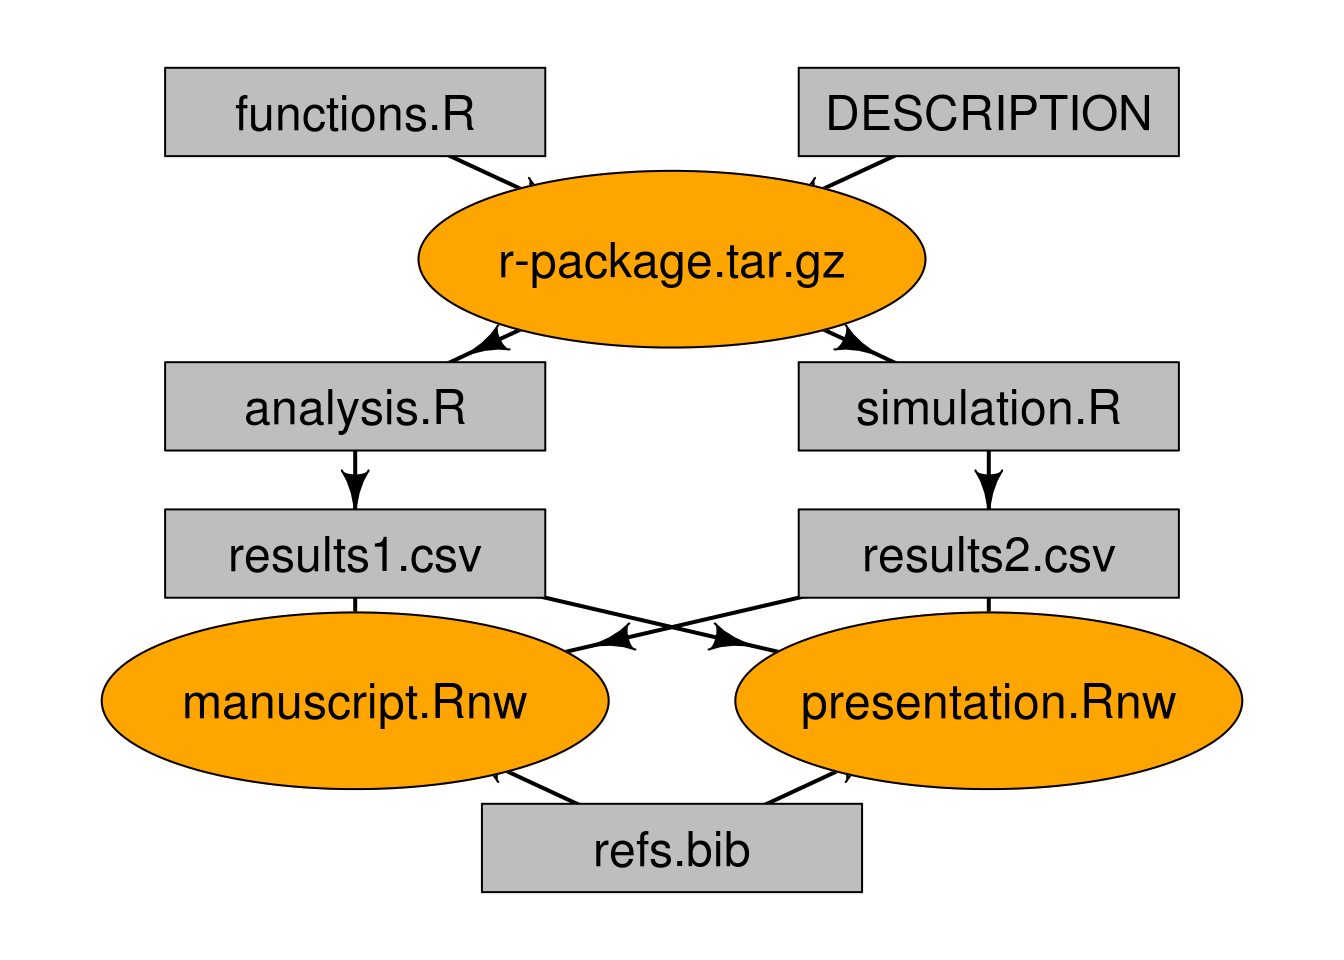
\includegraphics{10-build-automation_files/figure-latex/workflow-diagram-1.pdf}
\caption{\label{fig:workflow-diagram}Example project workflow}
\end{figure}

Re-running, -building, and -compiling all the files after we made a
change to the anyone of the intermediate files would be a tedious task.
Ideally, we would like to have a command that re-runs/compiles/builds
the different files everytime an upstream change is made. This is
exactly what the GNU software Make does. Make works through a Makefile,
a file that describes how a target file, depends on its dependencies,
and how these in turn on their dependencies, and so on. If a Makefile is
run, a file is compiled if any of its dependencies has changed since the
last time the file was compiled. In other words, the Makefile starts at
the top of the hierarchy and updates a file if its creation time is
older than the creation time of its dependencies. In our example in
Figure \ref{fig:workflow-diagram}, if we make a change to the
functions.R file, we trigger the recompilation of the recompilation of
the r-package.tar.gz file, which in turn triggers a rerunning of the
analysis.R and simulation.R scripts, and so on, until all files are up
to date again.

{[}add example Makefile{]}

\chapter{Dependency management}\label{dependency-management}

Reproducible research, in the narrow sense in which it is defined in
this book, ultimately means that an entire analysis - however
complicated - can be repeated at the push of a button (or the command
line equivalent: typing `make') to yield the exact same figures, tables,
files, or reports when aplied to the exact same data. In mathematical
terms, one could go as far as requriing that an analysis must act as a
function on data: there may very well be two data sets that produce the
same output but the same input data must always produce the same
analysis results. The core tools for achieving this are certainly
literate programming, which allows to closer integrate documentation and
code from a documentation-first perspective, and any form of build
automation/workflow management system (GNU make, snakemake, CWL, etc.).

It is certainly worthwhile to take a step back here and reflect on the
complexity of the approach that was put forward so far. None of the
steps suggested is excessively complex or requires a particularly deep
understanding of `the command line' but in combination a sizeable stack
of software dependencies has piled up:

\begin{enumerate}
\def\labelenumi{\arabic{enumi}.}
\tightlist
\item
  On the base layer, there is the operating system itself.
\item
  The analysis is conducted by interacting with the operating system,
  ideally, via some form of terminal and shell.
\item
  Next, a workflow management system or build system like GNU make,
  snakemake, or CWL-runner should be used to `tie everything together'
\item
  Version control softwae (usually git) is required to ensure integrity
  of the project
\item
  Usually some form of output is to be produced and the most reliable
  way to preserve digital documents at the moment seems to be .pdf. Note
  that changes in html/browser support may lead to different depiction
  of the same html file over the years! To create this output one will
  typically rely on some form of literate programming which has further
  dependencies. In the case of Rmarkdown and pdf output that would be R
  + pandoc + LaTeX.
\item
  Finally, the analysis itself will require even more complex software
  (R packages, python modules). In a scientific context there might also
  be bleeding edge software with no stabel release at all, which needs
  to be build from source.
\end{enumerate}

All in all, this software stack is incredibly complex even for the
simplest of analyses! Over time, each of these component layers might
change/be updated at different pace or the developmet might simply
cease. This situation can be pictured as a completed analysis being a
delicate skyscraper: the moment it is finished it starts to slowly
crumble away. {[}picture lening tower of pisa{]} Even if all all scripts
and report files were preserved exactly in the state they were in when
the analysis was conducted, the slowly evolving software ecosystem
around them will still change over time and it might very well be that
the excat same code would produce different results, or much more
likely, simply stop working at some point.

It is thus not enough to simply maintain a versioned repository of all
analysis scripts. Rather, complete reproducibility also requires a
perfect snapshot of the software environment at the time of execution to
be preserved for future execution - a time capsule of code if you will.
A good first step in this direction is certainly to report as many
version numbers of software used as possible. This approach, however, is
cumbersome, error prone and ultimately futile since users are typically
not even aware of the phletora of low level software they implicitly
rely on. A better approach would be to define explicitly the computing
environment required for the intended computation and to preserve an
exact `image' of this environemnt which can then be replicated at a
later point in time to re-run the analysis in it's original environment.

\section{Example problem}\label{example-problem}

Consider the toy example in
\url{https://github.com/rr-mrc-bsu/containerization-example}. This
example repository is build around a single R Markdown report
(\texttt{r-and-python.Rmd}) highlighting how R and python can be
integrated in a single report. While this is still a fairly simple
project in terms of dependencies (no custom source dependencies) it is
complex enough to highlight the benefits of a containerized analysis.

Let's sort throught the individual files and folder one by one. Any
well-organized repository should contain \texttt{README.md},
\texttt{LICENSE}, and \texttt{.gitignore} files. Their respective roles
are described in the git chapter {[}write chapter, REFERENCE{]}.

The \texttt{.travis.yml} configuration file contains the configuration
of the continuous integration system (here: Travis-CI) linked to the
repository. Continuous integration services allow automatic
builds/checks of the code in a repository and greatly facilitate quality
checking of new pull requests. To avoid a lengthly configuration file,
the folder \texttt{.travis} contains further scripts which are
referenced from the actual Travis configuration file. For details on
continuous integration, see chapter \ref{chptr-continuous-integration}.

The \texttt{Makefile} and the \texttt{Snakemake} files are explained in
more detail in chapter \ref(chpt-workflow-automation). These files can
be used to organize complex workflows using either GNU make (in simpler
cases) or snakemake (more sophisticated, cluster integration). We will
discuss how these two common workflow automation systems can be used
together with containers at the end of this chapter in section
\ref{sct-container-workflow-manager}.

The folder \texttt{mnist} contains prepared data from the classical
\href{http://yann.lecun.com/exdb/mnist/}{mnist} digital handwritten data
set.

The R Markdown file \texttt{r-and-python.Rmd} and the \texttt{docker}
folder are the elements of the example repository most important to the
contents of this chapter. The R Markdown file \texttt{r-and-python.Rmd}
contains an example analysis using python and tensorflow + keras to do
the heavy lifting for training a deep neural network to classify the
mnist example data (in digits 0 to 9). Some data wrangling and plotting
is done using R though. Both R and python sessions interoperate using
the \href{https://github.com/rstudio/reticulate}{\textbf{reticulate}
package}. To learn more about the language agnostic nature of R Markdown
and especially python/R interoperability, see {[}write chapter,
REFERENCE{]}. The analysis thus has a non-trivial set of dependencies in
both R and python packages/modules, which we will manage by using a
custom docker conatainer. The build instructions for this container are
specified in the \texttt{docker} folder which contains a build script
\texttt{docker/build} and a \texttt{dockerfile}. We will return to this
folder in section \ref{sct-docker}. Before learning more about
containers, it is a good idea to have a rough understanding of so called
`virtual machines'.

\section{Virtual machines and
containers}\label{virtual-machines-and-containers}

A virtual machines are (software) emulations of entire computer systems.
As such they allow running various guest operating systems from withing
a single host system, e.g., Linux within Windows or vice versa. To
achieve this, a virtual machine acts as intermediate layer between the
host system (and its hardware) and the guest operating system. I.e., all
low-level operatons of the guest system are mapped through the virtual
machine and the host operating system to the host hardware. A common
software for running virtual machines is
\href{https://www.virtualbox.org/}{VirtualBox} which can, e.g., be used
to run an Ubuntu linux from within a Windows system. When using virtual
machines for reproducible reseach, care should be taken to make the
process of creating the virtual machine as transparent as possible.
Command line tools like \href{https://www.vagrantup.com/}{Vagrant} are
much better suited for theses use cases. We strongly discourage setting
up a full-fledged Ubuntu system within VirtualBox and installing
required software manually from within the virtual machine since this
process is itself not reproducible. A virtual machine created in this
way may render a particular piece of code reproducible but can itself
not easily be recreated to the exact same specifications.

Instead, the reproducible research community is mainly embracing
containers to create portable computing environments. For our purposes,
containers can bee seen as a more leightweight alternative to virtual
machines. Snakemake {[}write chapter, REFERENCE{]}, for instance,
supports running workflows where individual steps are executed in their
respective individual containers.

\begin{quote}
In a nutshell, we may see container images as lightweight portable
pieces of software which can be used to spawn container instances thus
creating a \textbf{portable computing environment} by simply
distributing the respective container image file.
\end{quote}

If all dependencies of a particular analysis or an individual step in a
larger workflow are contained in a container image, these dependencies
will be available in any instance spawned from the image. An excellent
video explaining the concept of a container in more detail is:

\begin{itemize}
\tightlist
\item
  Ben Corrie, `what is a container?':
  \url{https://www.youtube.com/watch?v=EnJ7qX9fkcU}
\end{itemize}

By far the most common container software is Docker.

\subsection{Docker}\label{sct-docker}

\href{https://www.docker.com/}{Docker} constitutes the de-facto standard
in terms of container software and hugely contributed to popularizing
the concept of containerization in recent years. As most of the tools
discussed in this book, Docker was nnever designed with reproducibility
in mind but rather to enable the fast spinning-up of leightweight
application containers to handle web-services etc. (`micro
virtualization').

Since it is the de-facto standard, Docker is very well documented and t
he docker community edition is an open source project and available free
of charge. The company behind Docker als runs an online repository,
\href{https://www.docker.com/products/docker-hub}{Docker Hub}, for
docker images which can be seen as the GitHub/GitLab equivalent for
docker images. Docker Hub can be used free of charge and thus enables
the storage and sharing of custom container images via the world wide
web.

A major drawback of Docker is, that it was never intended as a
user-space application but mainly as a tool for server administrators.
As such it requires root access to operate. While this is fine for
buidling containers from so called \texttt{dockerfiles} (cf.
\texttt{docker/dockerfile} in the exampel repository), the execution of
an analysis should not require root access of the user. This is
especially important when computations are conducted on shared resource
like HPC systems where users do not have root access.

\subsection{Singularity}\label{singularity}

Only relatively recently, the \href{https://www.sylabs.io/}{singularity}
container software was introduced to address this issue. Singularity was
created exactly with HPC sytems and reproducibility in science in mind
(see \href{https://www.youtube.com/watch?v=DA87Ba2dpNM}{this} video{]}.
It does not require root access to run (but to build container images!)
and thus enables HPC users to locally build container images which they
can then use to run analyses on a high-performance cluster. A guiding
pricipal in the development of singularity was to maintain compatibility
with docker containers, i.e., singularity can be used to run standard
docker containers. Since singularity is still rather a niche product,
community help for docker is much easier to get online, and dockerhub is
arguably the safest (and cheapest) place to store and distribute
container images we still propose to use Docker for building the actual
container images.

\section{The dockerfile}\label{the-dockerfile}

A \texttt{dockerfile} contains the `recipe' for building a docker
container image. The complete reference of the syntax of dockerfiles can
be found \href{https://docs.docker.com/engine/reference/builder/}{here}.
For our purposes, only a few commands will suffice to set up a docker
container that contains all dependencies needed to render the Rmarkdown
file \texttt{r-and-python.Rmd} of the example project. In fact, the
entire contents of \texttt{docker/dockerfile} boil down to:

\begin{verbatim}
FROM rocker/verse:latest

MAINTAINER Kevin Kunzmann kevin.kunzmann@mrc-bsu.cam.ac.uk

# update apt
RUN sudo apt-get update

# install python and required packages
RUN sudo apt-get install -y python3-pip python3-dev python3-tk
RUN sudo pip3 install -U pip
RUN sudo pip3 install numpy matplotlib tensorflow

# install required R packages
RUN R -e "install.packages('reticulate')"
\end{verbatim}

Only three statements are used.

\begin{enumerate}
\def\labelenumi{\arabic{enumi}.}
\tightlist
\item
  The \texttt{FROM} statement indicates the basis of the container. This
  allows to build on existing containers which may then be modified or
  extended to save time and storage space since images are composed of
  individual layers. By re-using previous layers with \texttt{FROM} the
  respective layer must only be saved once per container repository.
  Here, the container is derived from the latest version of
  \href{https://www.rocker-project.org/}{\texttt{rocker/verse}}, a
  relatively large container consisting of a stable debian linux system
  with R, Rstudio, the tidyverse packges, and all software required to
  render Rmarkdownr reports (LaTeX) pre-installed.
\item
  The \texttt{MAINTAINER} field simplycontains an email address to
  complain to.
\item
  The \texttt{RUN} statement can be used to execute commmands inside the
  container during the build. Here we use it to update the distibution
  package manager before installing the R package \texttt{reticulate}
  which enables interoperability between R and python before installing
  python and the required modules.
\end{enumerate}

We will now build the container image locally. To that end, clone the
example repository to your local filesystem (cf. {[}TODO; REFERENCE
GIT{]}).

\begin{Shaded}
\begin{Highlighting}[]
\FunctionTok{git}\NormalTok{ clone https://github.com/rr-mrc-bsu/containerization-example}
\end{Highlighting}
\end{Shaded}

Next, \href{https://docs.docker.com/install/}{install docker},
\texttt{cd} to the docker subfolder of the example repository and build
the container via

\begin{Shaded}
\begin{Highlighting}[]
\BuiltInTok{cd}\NormalTok{ containerization-example/docker}
\FunctionTok{sudo}\NormalTok{ docker build --no-cache -t mycontainer .}
\end{Highlighting}
\end{Shaded}

Note that you do require root access to build the container! This
command will trigger the build process (and take a while). Afterwards, a
success message is displayed together with a unique
\href{https://en.wikipedia.org/wiki/SHA-2}{sha256 hash} value for the
container image. This hash value can later be used to uniquely identify
a particular versions of a container (similar to git commit hashes, cf.
???). Should you have a Docker Hub account you could then push the image
by

\begin{Shaded}
\begin{Highlighting}[]
\ExtensionTok{docker}\NormalTok{ push yourname/mycontainer}
\end{Highlighting}
\end{Shaded}

These are essentially the steps executed in the \texttt{docker/build}
script. WIthout making an image publicly available on dockerhub, the
image is only available locally. Note that having access to the image
(or at least its exact hash) is extremely important to guarantee
reproducibility. Simply rebuilding the image from the same dockerfile at
a later timepoint will almost always result in a slightly different
image when the build is configured to use the most recent package
sources and versions of the software required. To avoid this, one may
take steps to specify the software versions explicitly in the dockerfile
but this never guarantees reproducible builds due to the many
uncontrollable external dependencies. Still, keeping the dockerfile is
important, since it may be seen as a guide as to how a similar computing
environment can be set up manually at a later timepoint. Even if there
are reasons not to use singularity to re-run an analysis, as good
dockerfile might be the best way to specify software dependencies.

{[}TODO link to continuous integration for dockerfiles{]}

Switch back to the top level of the containerization example folder now.

\begin{Shaded}
\begin{Highlighting}[]
\BuiltInTok{cd}\NormalTok{ ..}
\end{Highlighting}
\end{Shaded}

A major advantage of singularity over docker over virtual machines is
the ease with which singularity enables execution of commands
\textbf{inside of a docker container instance} but \textbf{within the
host file system}, i.e., in contrast to docker, one does not need to
manually mount a particular directory when starting a container but
simply may invoke

\begin{verbatim}
singularity exec docker://kkmann/rr-containerization-example touch test
\end{verbatim}

to execute the command \texttt{touch\ test} in an instance of the
publicly built container image but \textbf{within the host filesystem}.
This means that after executing the line in a shell, a new file `test'
should have been created in the current working directory. The touch
command, however, was not executed in the host system but within the
container! This example is obviously useless since \texttt{touch} is
just as well available in the host shell but it immediately demonstrates
the ease of using singularity with the host file system!

\section{Containers and workflow
management}\label{sct-container-workflow-manager}

\subsection{GNU make}\label{gnu-make}

A much more useful application in our context is executing GNU make in a
container! This means that we can render the Rmarkdown file in our
container by

\begin{Shaded}
\begin{Highlighting}[]
\ExtensionTok{singularity}\NormalTok{ exec docker://kkmann/rr-containerization-example make}
\end{Highlighting}
\end{Shaded}

Since all dependencies are pre-installed in the container image, this
command only depends on the verson of singularity and the exact
container image. To query the exact sha256 hash value, use
\texttt{docker\ images}

\begin{Shaded}
\begin{Highlighting}[]
\ExtensionTok{docker}\NormalTok{ images --digest }\KeywordTok{|} \FunctionTok{grep}\NormalTok{ containerization}
\end{Highlighting}
\end{Shaded}

which will list the locally available corresponding container images and
there exact hash values. To re-use a particular version, one may then
invoke, e.g.,

\begin{verbatim}
singularity exec docker://kkmann/rr-containerization-example@sha256:5225e53f934d749bf3017f140e5169b0d2eadc0512799b89c2f854a2d002d0c4 make
\end{verbatim}

\subsection{Snakemake}\label{snakemake}

Snakemake is a much more powerful tool whe it comes to complex workflows
since it supports cluster execution and more flexible rule definitions
(cf chapter {[}TODO, REFERENCE{]}). It is also designed with
reproducibility in mind and thus allows to run either specific rules or
an entire workflow using singularity. The contents of the
\texttt{Snakefile} in the containerization-example folder are

\begin{verbatim}
singularity:
    "docker://kkmann/rr-containerization-example@sha256:17414f63929b0283f82e70ded3ca9cd9b61f37e13fe3d103a2bdf24b9056114e"

rule build_report:
    input:
        "r-and-python.Rmd"
    output:
        "r-and-python.html"
    shell:
        """
        Rscript -e "rmarkdown::render(\\"{input}\\")"
        """
\end{verbatim}

The first line specifies the singularity container to use. Here, the
publicly available image from dockerhub is used with a particular hash
value. One could just as well point to a local image as well though.
Such a global singularity parameter will run every rule of the workflow
in the same default container. It is also possible to specify custom
containers on a per-rule basis by specifying the \texttt{singularity}
parameter of the rule.

\begin{verbatim}
rule build_report:
    input:
        "r-and-python.Rmd"
    output:
        "r-and-python.html"
    singularity:
        "docker://kkmann/rr-containerization-example@sha256:17414f63929b0283f82e70ded3ca9cd9b61f37e13fe3d103a2bdf24b9056114e"
    shell:
        """
        Rscript -e "rmarkdown::render(\\"{input}\\")"
        """
\end{verbatim}

This will override potential gloabl singularity container settings (cf.
{[}REFERENE SINGULARITY CHAPTER{]}).

\section{Containerization vs.~package
managers}\label{containerization-vs.package-managers}

The approach to dependency management presented in this chapter might be
considered a bit overpowered for some use cases. The main reason why we
chose to demonstrate what we consider the `gold-standard' of dependency
management over more language/environment specific approaches is to is
to showcase how simple it actually is. As long as you are capabale of
running a few simple commands in a linux command line you are good to
go. The container-based approach to dependency managemnt is also the
most generic in that it is capable of managing arbitrary dependencies -
as long as your computing environment can be set up on a linux operating
system you are good to go! It does not matter which (or even how many
different) programming languages you use, how much messy custom research
software you need. As long as you are able to install it to a plain
linux system there is no environment that cannot be mapped to a
container (or several!). Still, for completeness' sake, a few different,
potentially more accessible methods for partial dependency management
will be discussed as `honorable mentions' in the following.

\subsection{R only - wrap everything up in a
package}\label{r-only---wrap-everything-up-in-a-package}

In case your entire workflow is R-based, it might be worthwhile to write
an R packge for your analysis. This essentially relies on R's package
management system to resolve dependencies (in this case: R packages
only). An R analysis package tends to not contain much code in the
\texttt{R/} folder, but rather encapsulates any analyses in vignettes.
{[}TODO: elaborate on this idea, example repository{]}

\subsection{R only - packrat}\label{r-only---packrat}

{[}TODO{]}

\section{Caveats}\label{caveats}

Depending on your perspective, there are a few restrictions to a
container-based dependency management approach.

\begin{enumerate}
\def\labelenumi{\arabic{enumi}.}
\tightlist
\item
  \textbf{Licensing:} Reproducibility and the open-source philosophy are
  closely connected in that true reproducibility requires the software
  dependencies to be openly available. If the required dependencies
  cannot be installed in a container that may be distributed openly,
  results will not be reproducible by everybody. For instance, while the
  SAS system for statistical analyses can be used inside containers,
  licensing and license consts may be a major obstacle in doing so.
\item
  \textbf{Containers are linux based:} The effective restriciton to
  open-source software also restricts the choice of container operating
  systems. In practice, containers are almost exclusively linux based.
  In case of, e.g., Windows dependencies, this means that the less
  flexible approach via virtual machines might be required to
  encapsulate the analysis environment.
\end{enumerate}

While these restrictions might be seen as caveats, in fact, they can
also be seen as an encouragement to conducting research in a more open
(as in open-source-software-based) way.

\chapter{Continuous Integration}\label{chptr-continuous-integration}

Did you ever wonder what the green/yellow/red `badges' in some Readme.md
files on, e.g., Github.com actually mean? How are they created, what are
they for and why should you care?

This section will hopefully shed light on the meaning of some of these
badges (those refering to a `build status') and you will learn how to
use these techniques for you own repositories. The key term here is
`continuous integration' (CI) which refers to a concept in software
development where all working copies (in git one would refer to
branches) of a project are frequently integrated into the mainline (in
git terms: the master branch). The rationale being that
frequent/continuous integration prevents diverging development branches.
Since the philosophy of git is to create feature branches for small,
contained changes of master which are to be merged back as soon as
possible CI and git are a natural fit.

In practice, however, frequent changes to master are dangerous. After
all, the master branch should maintain the last at least working if not
stable version of the project that other feature branches can be started
from. It is thus crucial to prevent erroneous changes to be merged into
the master branch too often. This means that CI requires some kind of
automated quality checks that preemptively check for new bugs/problems
before a pull request from a feature branch on master is executed. It is
this particular aspect of CI that is most interesting to collaborative
work on scientific coding projects - being able to automatically run
checks/tests on pull requests proposing changes to the master branch of
the project.

{[}Random thought: we should have an example repository for
demonstraiting the different states of PRs etc. instead of just
including pictures. Readers could then inspect the `frozen' repository
directly and see the PRs etc.!{]}

To enable this kind of feature on Github, a cloud-based farm or build
servers is required where users can run build scripts in virtual
machines and retrieve reports on the build status (0 worked, 1 failed).
It is these build-statuses that the green/yellow/red badges report
visually (yellow/gray being a pending build)! There are multiple
companies offering these services (within reasonable bounds) for free
for public repositories and as of 2018 the free academic account for
GitHub also enables free builds using TravisCI for private repositories.
It must be stressed though that, since everything is running in the
cloud, the same constraints as for storing data on GitHub servers apply
to downloading or processing data in buildscripts for CI services.
{[}point to Jenkins as on-premis solution{]}

The obvious setting to use automated builds in is package development.
This is by far the most common application and the current tools are
definitely geared towards that use case. We will later discuss how to
extend the scope to non-package situations. For instance, the repository
containing the source code for this book also uses TravisCI for build
automation even though it is not an R-package itself.

\chapter{Metadata}\label{chptr-metadata}

\begin{itemize}
\tightlist
\item
  what is metadata?
\item
  indexing and search engines?
\item
  long term storage/accessibility
\end{itemize}

\section{FAIR principle}\label{sct-fair}

{[}todo{]}

\section{Digintal Object Identifiers - DOI}\label{sct-doi}

{[}todo{]}

\section{Zenodo.org}\label{sct-zenodo}

{[}todo{]}

\chapter{R package development}\label{r-package-development}

\section{Continuous integration}\label{continuous-integration}

\section{Unit testing}\label{unit-testing}

\section{Documentation}\label{documentation}

\chapter{Python package development}\label{python-package-development}

\section{Continuous integration}\label{continuous-integration-1}

I agree, Kevin, we should some content.

\section{Unit testing}\label{unit-testing-1}

\section{Documentation}\label{documentation-1}

\bibliography{book.bib,packages.bib}


\end{document}
